\chapter{Installation}

\section{Prerequisites}

\begin{itemize}
\item This package aims at automating GSAS, therefore, a running GSAS is required. To test this, at the command line from which you wish to run this (mouse junkies - this will NOT be your cup of tea - but maybe we can pull you into the great land of command lines) change into a folder with GSAS data and try to plot it in rawplot by typing in rawplot. If this fails with a file not found error, GSAS is either not installed or not in the search path\footnote{On windows systems, go to the control panel, advanced setup, environment variables, and add "\texttt{;c:\textbackslash gsas\textbackslash exe}" at the end of the search path. On Unix systems, add ":/usr/local/gsas/exe" to you PATH variable in something like \texttt{\textasciitilde/.bashrc} or so.}. If it plots, but doesn't have text around the graph, the PGPLOT\_FONT variable is not set. Another missing bit could be the GSAS variable, in which case GSAS wouldn't know where to look for the scattering length etc. All this is documented somewhat in the README file coming with GSAS, but who reads those these days... Please note that PC-GSAS and EXPGUI are setting the environment variables only for the current session, that is enough for what we want to do here, so a running PC-GSAS or EXPGUI is not sufficient.
\item The 2nd prerequisite is a working understanding of GSAS by the user. If you don't know what GSAS does and how it works, this here will be of little help, it might be even dangerous due to the GIGO problem\footnote{garbage in, garbage out}... We strongly suggest you work at least through the excellent tutorials that come with GSAS to get an idea what GSAS does. To encourage that, the examples we provide here are the tutorials from the GSAS manual cast into scripts.
\end{itemize}

\section{Linux or Windows?}

We found that the same stuff runs faster when a given system runs under Linux. Here are some numbers on a 28 histogram refinement, including 8th order spherical harmonics texture. On both platforms, the same data was analyzed with the same script. The platform was a Dell Optiplex 960 (Quadcore Intel CPU, 3GHz, 4GB RAM). No other major tasks were running on the machine.

\begin{tabular}{|l|c|c|}
\hline
&Linux&Windows\\
\hline
OS&OpenSuse&Windows XP Professional\\
Version&11.2, Kernel 2.6.31.14-0.6 SMP&5.1.2600 SP3 Build 2600\\
total runtime [s]&2497&2652\\
average GENLES cycle time [s]&11.2(2.7)&12.4 (3.2)\\
Minimum GENLES cycle time [s]&4.1&4.8\\
Maximum GENLES cycle time [s]&18.5&20.1\\
\hline
\end{tabular}

On average, each GENLES cycle is 9\% faster when running Linux with a maximum improvement of 17\%. The overall runtime is reduced by 6.2\% when running Linux.

\section{Linux/Mac/Unix Installation}

\begin{itemize}
\item Download the zip file with the latest scripts from \url{http://code.google.com/p/gsaslanguage/}. 
\item Copy the scripts into an appropriate folder and add it to the path. Done.
\item Ok, maybe not completely. Make sure you have LaTex installed (punch in \texttt{latex} at a command prompt, it should come up with a LaTeX prompt). If you want to plot the results of a multi-run analysis using gsas\_plot\_overview, make sure you have gnuplot installed, try typing \texttt{gnuplot} at a shell prompt.
\end{itemize}

\section{Windows Installation}

This is a bit more lengthy since many of the Unix standard software, like a bash shell, latex and gnuplot don't come with the standard Windows.
\begin{itemize}
\item Copy the scripts into an appropriate folder, e.g. \texttt{c:\textbackslash gsaslanguage} 
\item Since we need a bash shell, install the cygwin package from (www.cygwin.com).  Download the setup executable and store it in the same folder where you will install cygwin (e.g. \texttt{c:\textbackslash cygwin} ). That way it can be used for future additions and updates. Provide your internet options. If you are working at a government lab, choose a cygwin site at another government lab (.gov) since they are connected with a high-speed backbone. Once you see the ``select packages'' screen (see screenshot below), click on the ``View'' button in the top right corner until you see the ``Full'' view. Besides the basic cygwin, select to install also gnuplot.  Make sure to follow the UNIX end-of-line convention, if in doubt (getting weird error messages when running the gsas scripts such as ``unexpected end of file'' or so), run ``dos2unix'' on your script from the command line.
\begin{figure}[h]
\centering
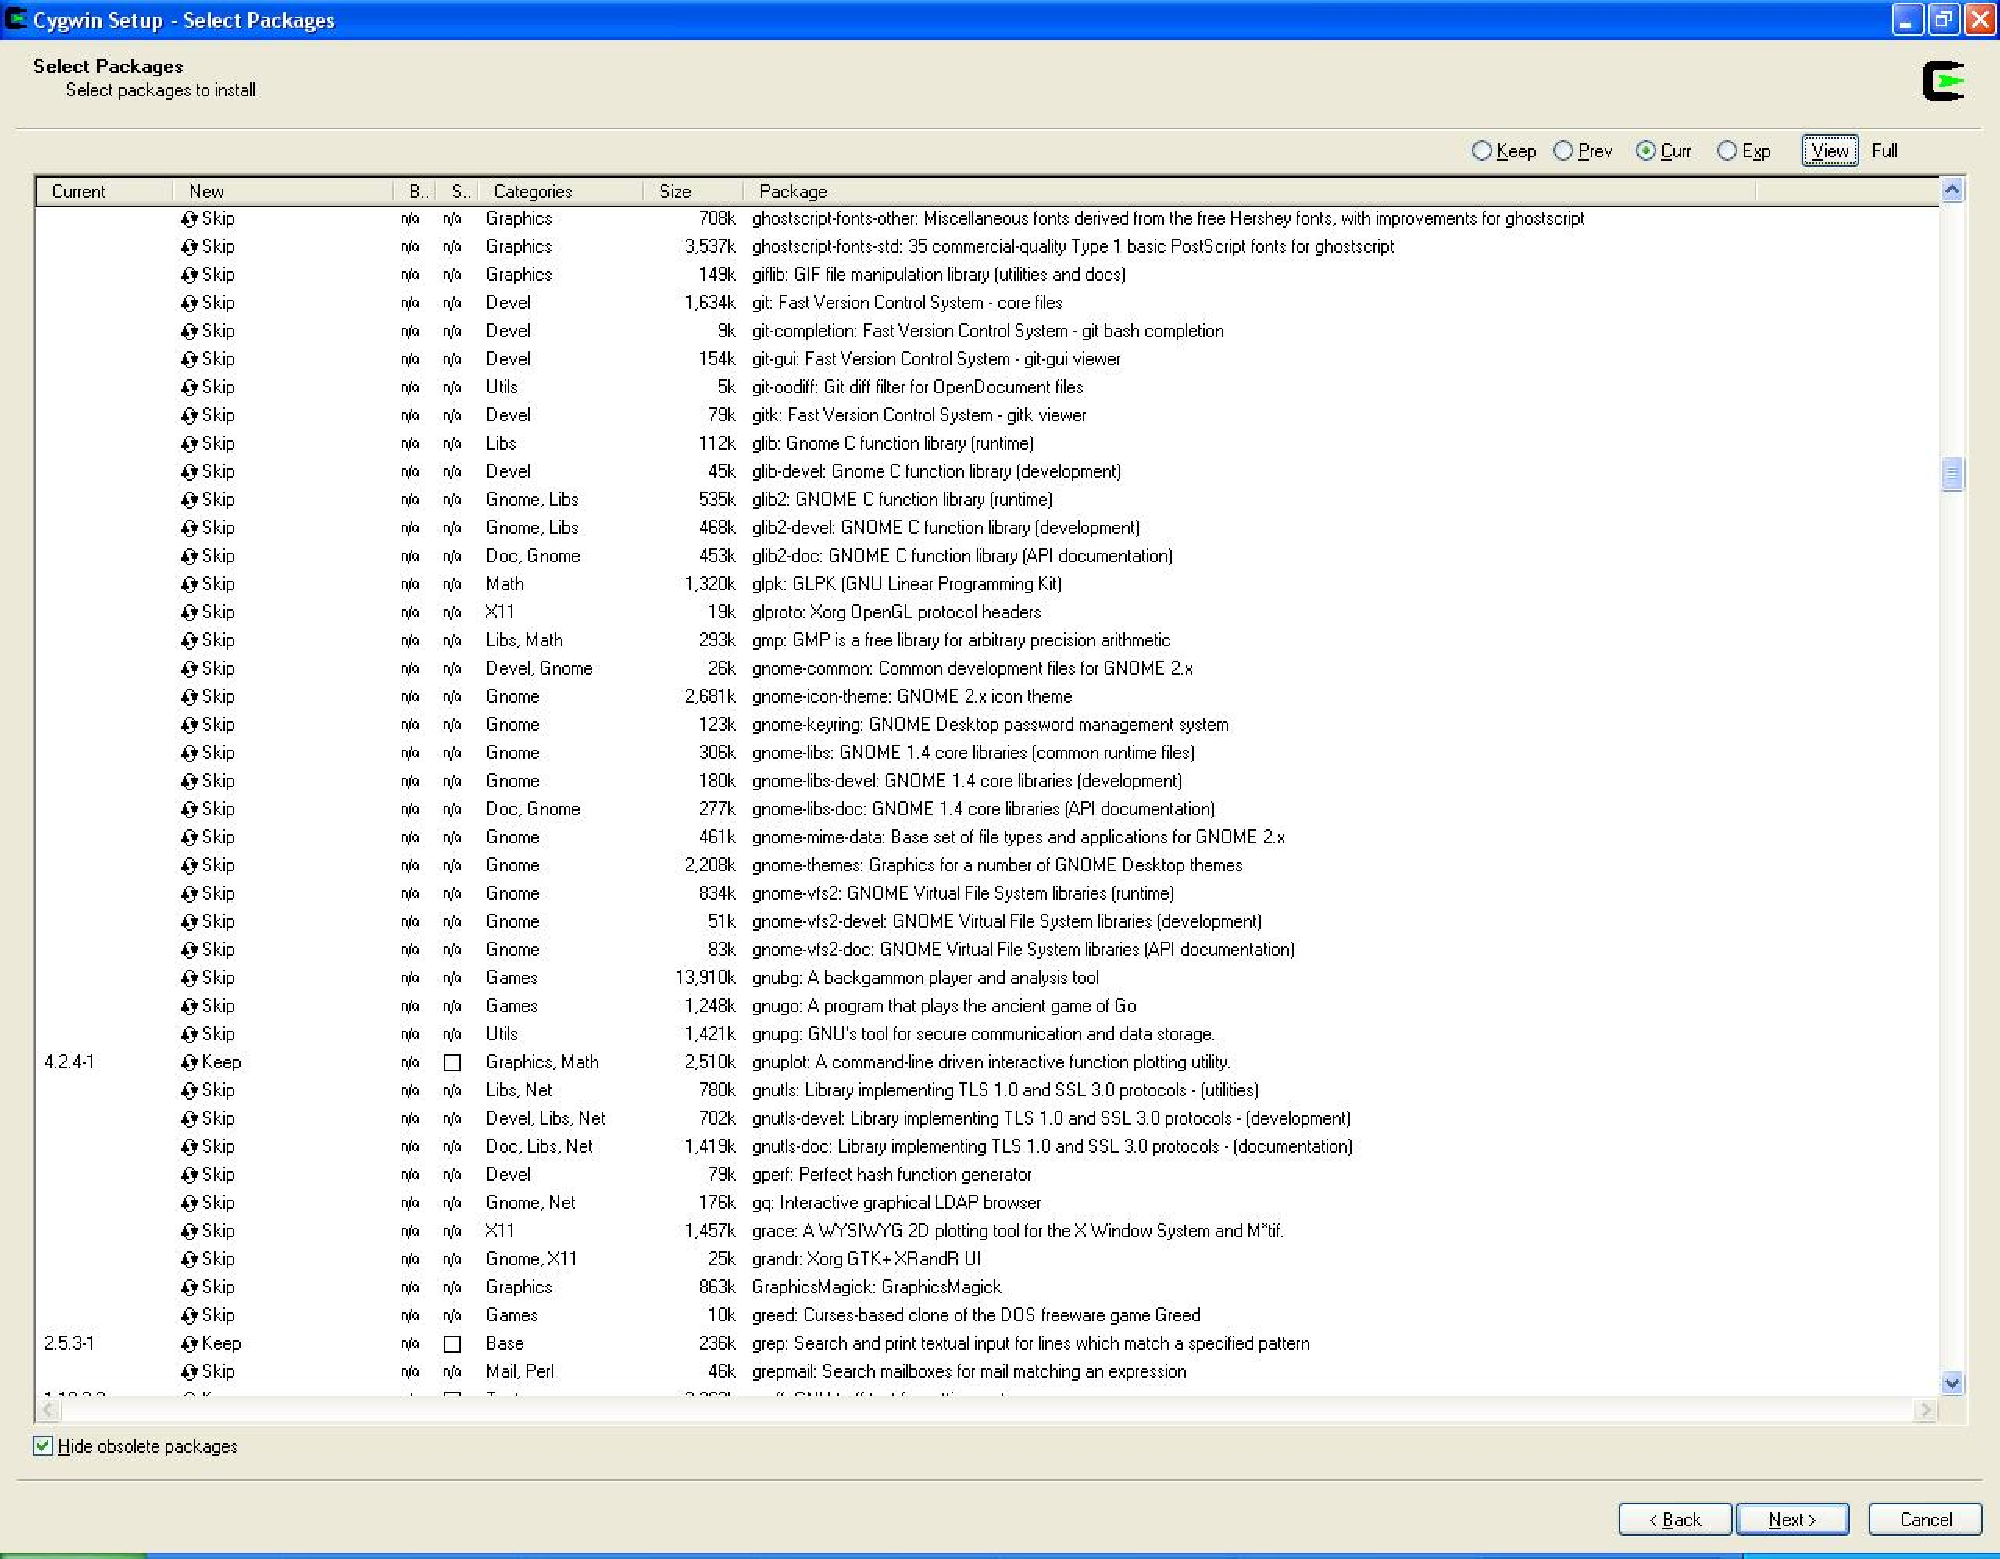
\includegraphics[width=12cm]{Screenshot1.pdf}
\caption{Selecting packages during Cygwin installation}
\label{fig:Screenshot1}
\end{figure}

\item Get the GSAS scripts from \url{http://code.google.com/p/gsaslanguage/}. Add the folder name to the search path (Control Panel -- System -- Advanced
-- Environment Variables -- PATH)
\item Install LaTex (go to miktex.org to download the basic installation for a Windows system).
\item You may have to install the LaTeX package fullpage manually if your firewall does not allow LaTeX to install it on the fly. If you are using Miktex (Basic MiKtex 2.7), install it into a subfolder of your Miktex installation and refresh the Filename database in the Miktex options.
\end{itemize}

